\section{Profiling}

\subsection{Education}
Variable Type: Categorical Nominal. 
Recall: the Education variable describes the level of studies the consumer has (2nd cycle, Basic, Graduation, Master, PhD).

\begin{figure}[H]
    \centering
    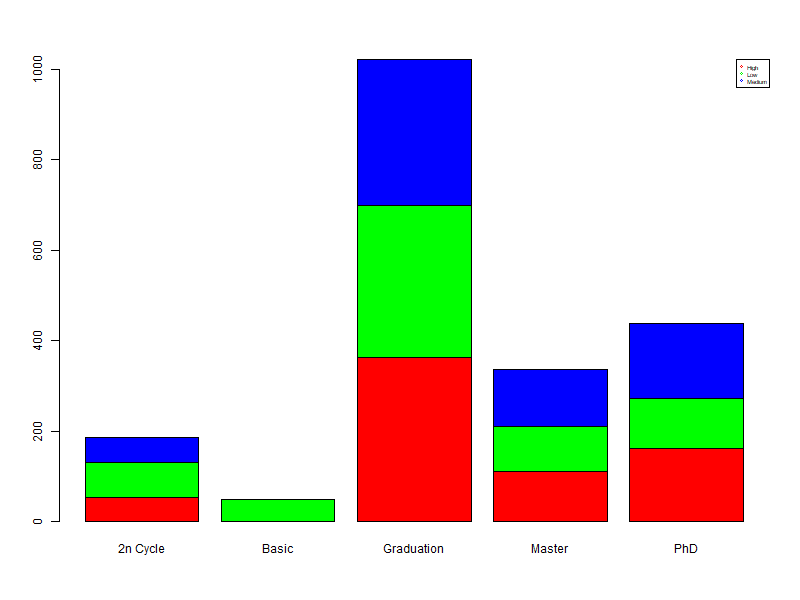
\includegraphics[width= 1\linewidth]{Imatges/stacked_barplot_counts_IncomeSegment_10_legend(education).png}
    \caption{Descripció}
    \label{fig:scree_plot_1} % Changed label to be unique
\end{figure}

This graph shows that most of the data comes from graduate consumers, while those with a basic education level are scarce. It also illustrates the income status for each education level, highlighting that the basic level stands out as the only one not evenly distributed.
\begin{figure}[H]
    \centering
    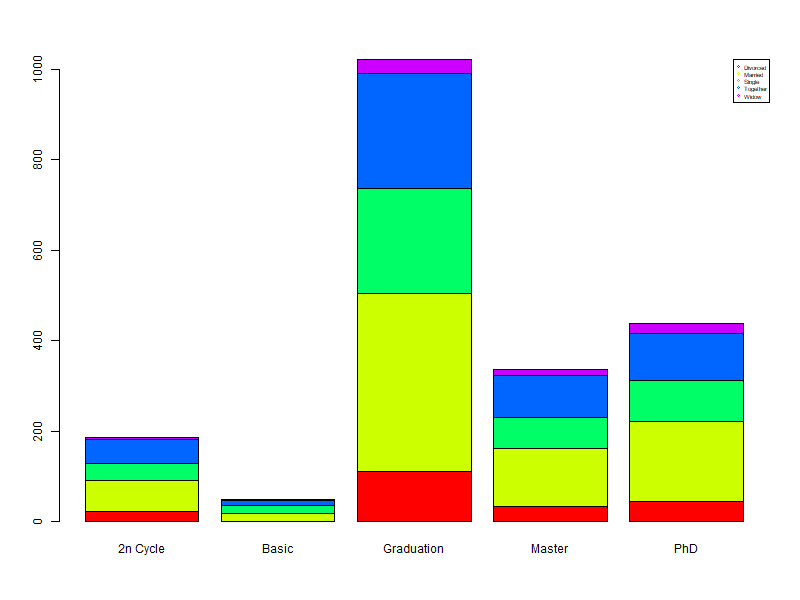
\includegraphics[width= 1\linewidth]{Imatges/stacked_barplot_counts_MaritalSts_10_legend(education).png}
    \caption{Descripció}
    \label{fig:scree_plot_1} % Changed label to be unique
\end{figure}

If we look at it according to marital status, we realize that most are married or in a relationship.

\begin{figure}[H]
    \centering
    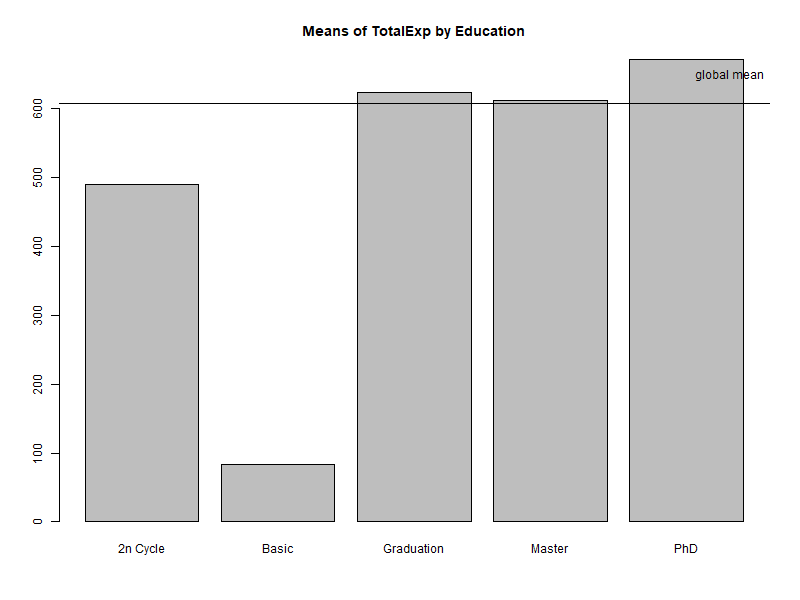
\includegraphics[width= 1\linewidth]{Imatges/mean_barplot_TotalExp.png}
    \caption{Descripció}
    \label{fig:scree_plot_1} % Changed label to be unique
\end{figure}

With a mean bar plot we can see the total expend depending on the level of studies, where it is evident that the basic education group spends much less money on their purchase.

\begin{figure}[H]
    \centering
    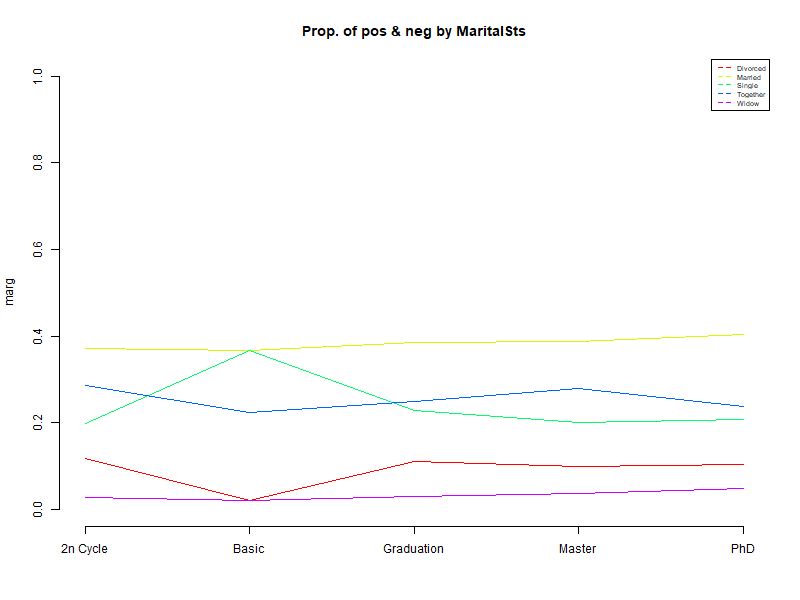
\includegraphics[width= 1\linewidth]{Imatges/prop_cond_class_MaritalSts_4_legend.png}
    \caption{Descripció}
    \label{fig:scree_plot_2} % Changed label to be unique
\end{figure}

Comparing with the marital status we can see that independently of their studies, the customers usually are married or together. It is worth noting that those with a basic education level are more often married or single.
\begin{figure}[H]
    \centering
    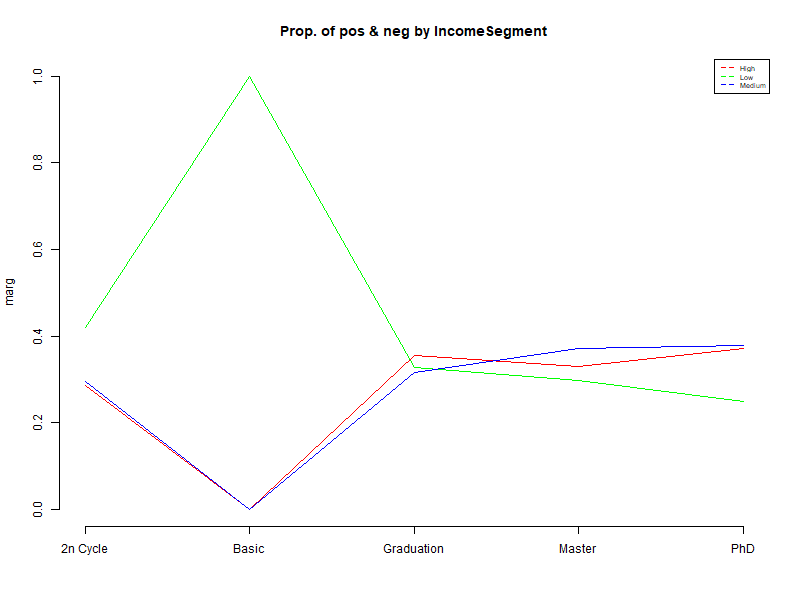
\includegraphics[width= 1\linewidth]{Imatges/prop_cond_class_IncomeSegment_4_legend.png}
    \caption{Descripció}
    \label{fig:scree_plot_3} % Changed label to be unique
\end{figure}

Comparing the income segment we can see that the basic level has the highest frequency with low segment. It shows that they are the ones with the lowest incomes, followed by those with a second-level education, and that there is not much difference among the rest.
\begin{figure}[H]
    \centering
    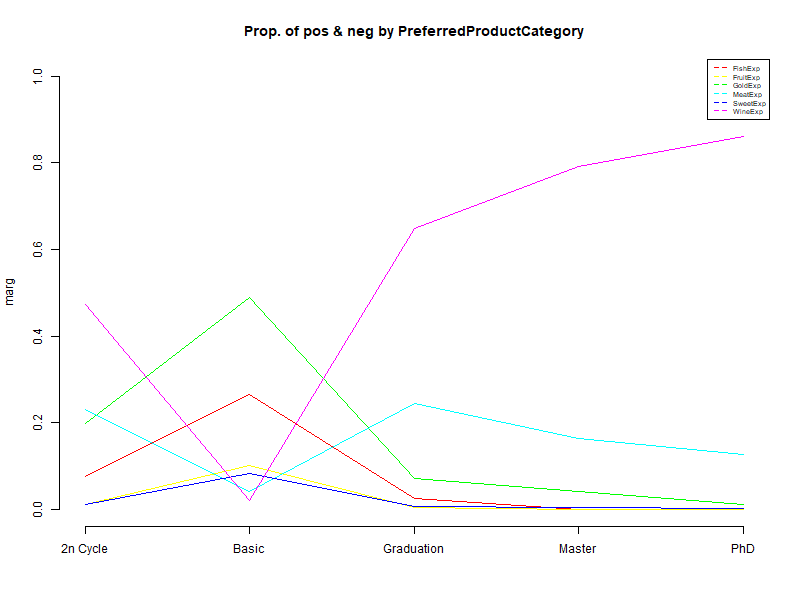
\includegraphics[width= 1\linewidth]{Imatges/prop_cond_class_PreferredProductCategory_4_legend.png}
    \caption{Descripció}
    \label{fig:scree_plot_4} % Changed label to be unique
\end{figure}

About their most purchased product category, we can see that as the level of education increases, there is a tendency to spend more on wine, the customers with lower education levels prefer to buy gold, and those with a graduation level education tend to spend on meat.

\newpage
\subsection{MaritalSts}
Variable Type: Categorical Nominal. 
Recall: the MaritalSts variable describes the marital status of the customer (Divorced, Married, Single, Together, Widow).

\begin{figure}[H]
    \centering
    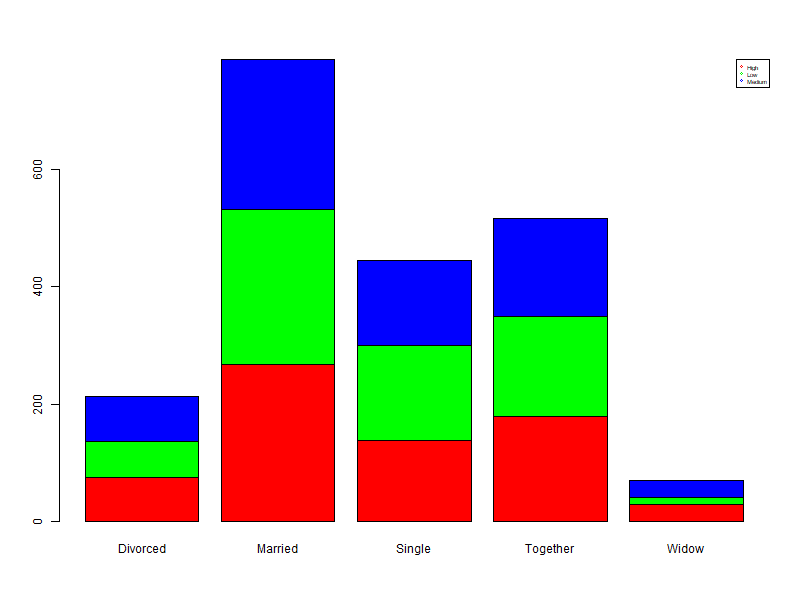
\includegraphics[width= 1\linewidth]{Imatges/stacked_barplot_counts_IncomeSegment_10_legend(marital).png}
    \caption{Descripció}
    \label{fig:scree_plot_5} % Changed label to be unique
\end{figure}

With this graph, we can see that income level is fairly consistent, so it does not seem to influence marital status.

\begin{figure}[H]
    \centering
    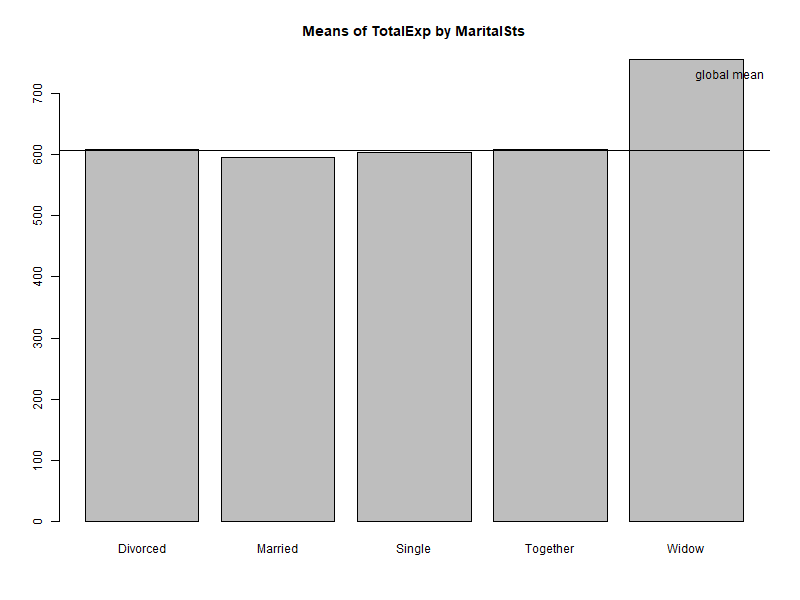
\includegraphics[width= 1\linewidth]{Imatges/mean_barplot_TotalExp(2).png}
    \caption{Descripció}
    \label{fig:scree_plot_5} % Changed label to be unique
\end{figure}

With a mean bar plot we can see that the total expenditure by marital status is quite uniform, despite widow customers that spends more on average.

\begin{figure}[H]
    \centering
    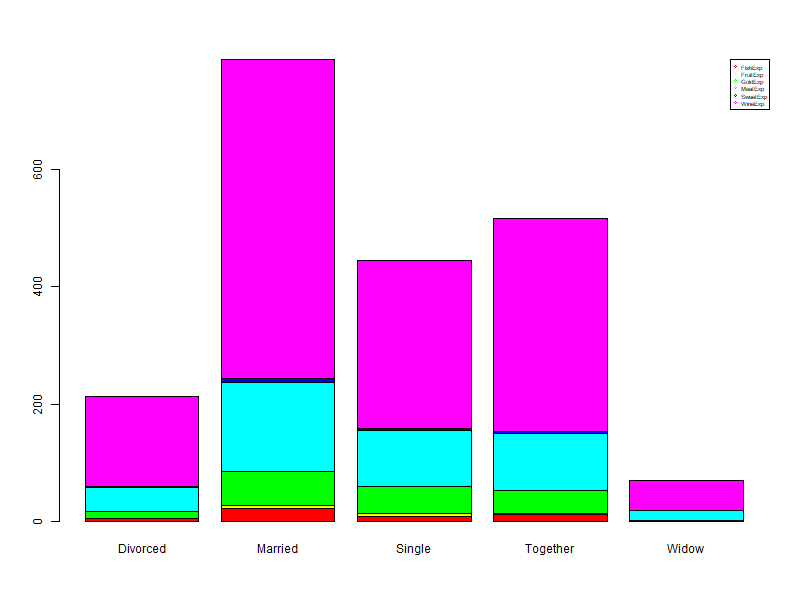
\includegraphics[width= 1\linewidth]{Imatges/stacked_barplot_counts_PreferredProductCategory_10_legend.png}
    \caption{Descripció}
    \label{fig:scree_plot_6} % Changed label to be unique
\end{figure}

It is interesting to observe that regardless of marital status, the main product is wine, followed by meat.

\newpage
\subsection{IncomeSegment}
Variable Type: Numerical Discrete. 
Recall: The IncomeSegment variable groups customers into 'Low' (blue), 'Medium' (green), and 'High' (red) income brackets.

\begin{figure}[H]
    \centering
    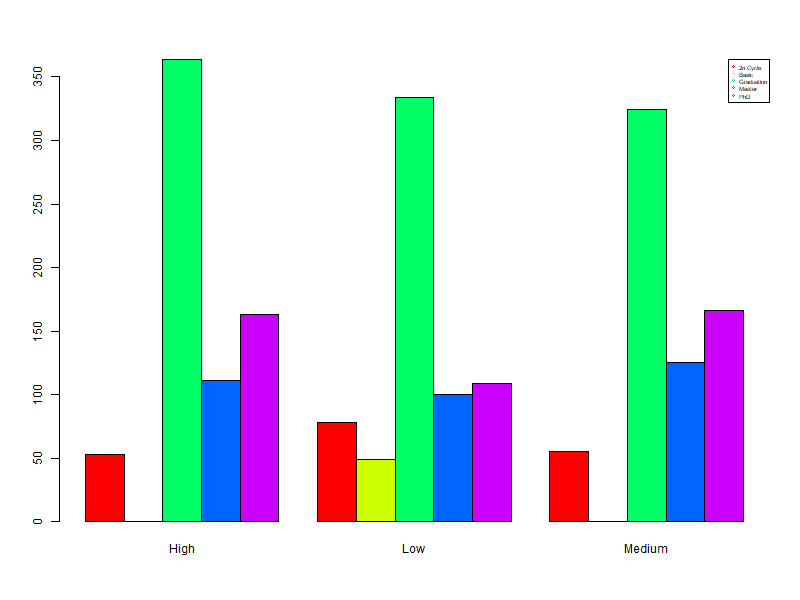
\includegraphics[width= 1\linewidth]{Imatges/grouped_barplot_counts_Education_12_legend(income).png}
    \caption{Descripció}
    \label{fig:scree_plot_7} % Changed label to be unique
\end{figure}

In this graph, we can observe in more detail the education levels that make up each income status. We can see that consumers are distributed in roughly the same proportion across the three cases; however, the basic level stands out because it only appears in the low-income status.


\begin{figure}[H]
    \centering
    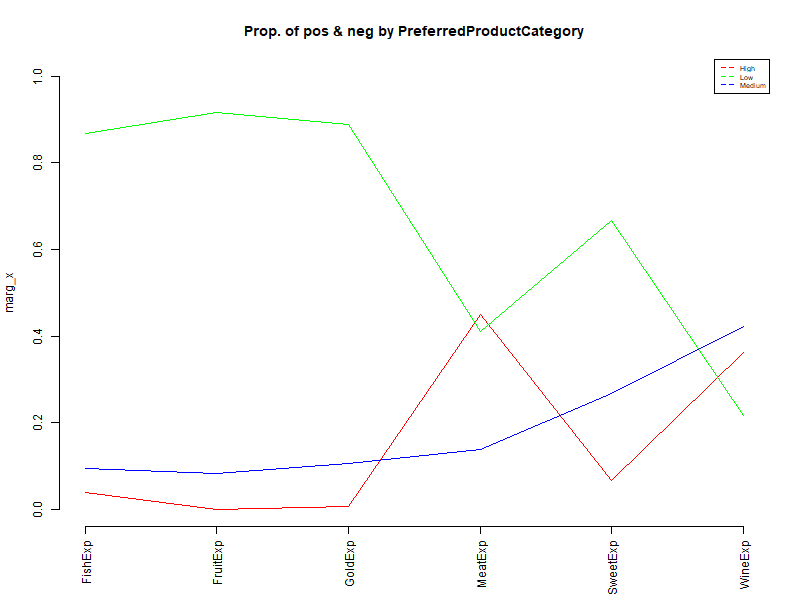
\includegraphics[width= 1\linewidth]{Imatges/prop_cond_col_var_x_PreferredProductCategory_8_legend.png}
    \caption{Descripció}
    \label{fig:scree_plot_7} % Changed label to be unique
\end{figure}

With this graph, it can be observed that the preferred category of customers varies depending on their segment. This shows how different their main interests are when it comes to spending their income.

\newpage
\subsection{HasChildren}
Variable Type: Categorical Binary. 
Recall: the HasChildren variable whether the customer has children or not (0 or 1).

\begin{figure}[H]
    \centering
    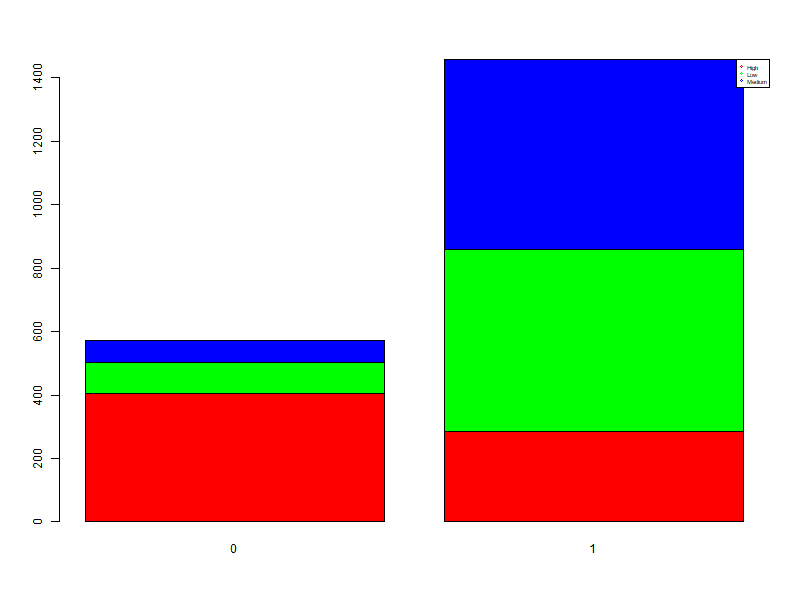
\includegraphics[width= 1\linewidth]{Imatges/stacked_barplot_counts_IncomeSegment_10_legend.png}
    \caption{Income Segment Counts by HasChildren (0 = No, 1 = Yes)}
    \label{fig:scree_plot_8} % Changed label to be unique
\end{figure}

This stacked bar chart provides a clear breakdown of income segments based on whether the customer has children (assuming '0' is No Children and '1' is Has Children).

The 'No Children' segment (bar '0') is the larger group overall (approx. 1150 customers) and is dominated by \textbf{High-income consumers} (red, approx. 630 counts), followed by Low-income (blue, approx. 370).

The 'Has Children' segment (bar '1') is smaller (approx. 820 customers) and is overwhelmingly composed of \textbf{Medium-income} (green, approx. 520) and \textbf{Low-income} (blue, approx. 250) consumers, with a very small High-income group (red).

This strongly suggests that having children is correlated with being in the Medium or Low income brackets, while not having children is associated with the High-income segment.

\begin{figure}[H]
    \centering
    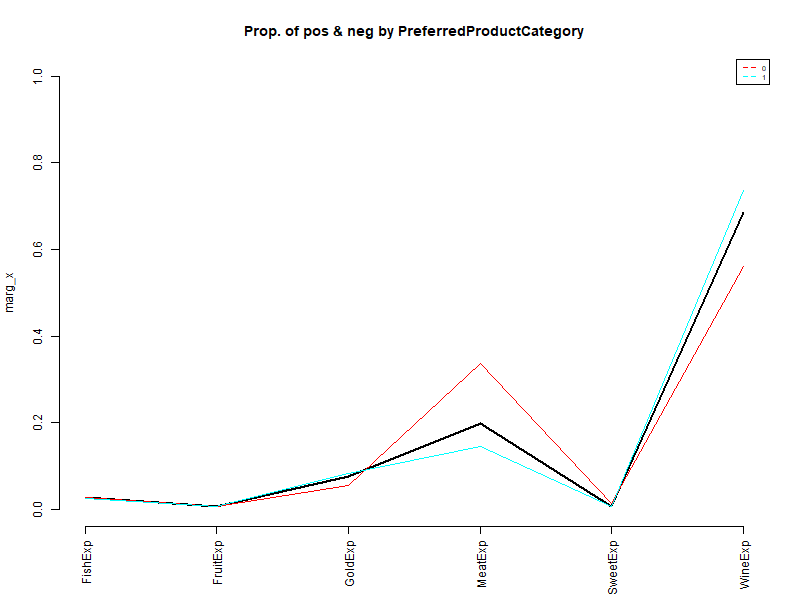
\includegraphics[width= 1\linewidth]{Imatges/prop_cond_class_var_x_PreferredProductCategory_6_legend.png}
    \caption{Proportional Preference by Product Category}
    \label{fig:scree_plot_9} % Changed label to be unique
\end{figure}

This line plot shows that product preference is \textbf{not affected} by having children. The preference proportions for customers with 'No Children' (red line, '0') and 'Has Children' (cyan line, '1') are nearly identical. Both groups overwhelmingly prefer \textbf{Wine}, with a secondary, smaller preference for \textbf{Meat}. All other categories show very low preference proportions for both segments.

\newpage
\subsection{PreferredChannel}
Variable Type: Categorical Nominal. 
Recall: the PreferredChannel variable describes the channel with highest frequency.

\begin{figure}[H]
    \centering
    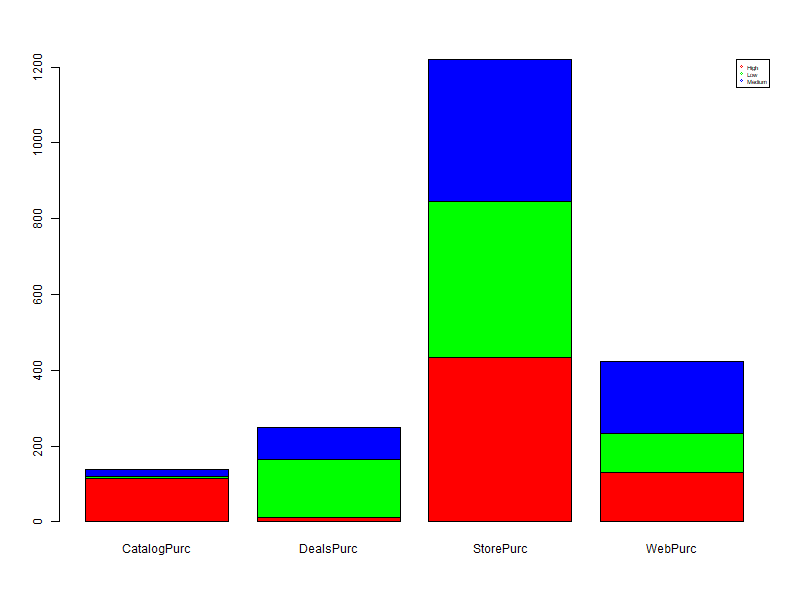
\includegraphics[width= 1\linewidth]{Imatges/stacked_barplot_counts_IncomeSegment_10_legend(channel).png}
    \caption{Preferred Channel by Income Segment}
    \label{fig:scree_plot_10} % Changed label to be unique
\end{figure}

This graph clearly shows that \textbf{'StorePurc'} (In-Store) is the most common preferred channel by a large margin, utilized heavily by all income segments. The other channels, however, reveal strong income-based preferences:
\begin{itemize}
    \item \textbf{CatalogPurc:} This is almost exclusively a \textbf{High-income} (red) channel.
    \item \textbf{DealsPurc:} This channel is dominated by \textbf{Low-income} (blue) and \textbf{Medium-income} (green) shoppers, with almost no participation from the High-income segment.
    \item \textbf{WebPurc:} Online shopping is also most popular with the \textbf{Low-income} (blue) segment, followed closely by the Medium-income (green) segment. The High-income segment shows the least preference for this channel.
\end{itemize}

\newpage
\subsection{PreferredProductCategory}
Variable Type: Categorical Nominal. 
Recall: the PreferredProductCategory variable describes the category with highest frequency.
\begin{figure}[H]
    \centering
    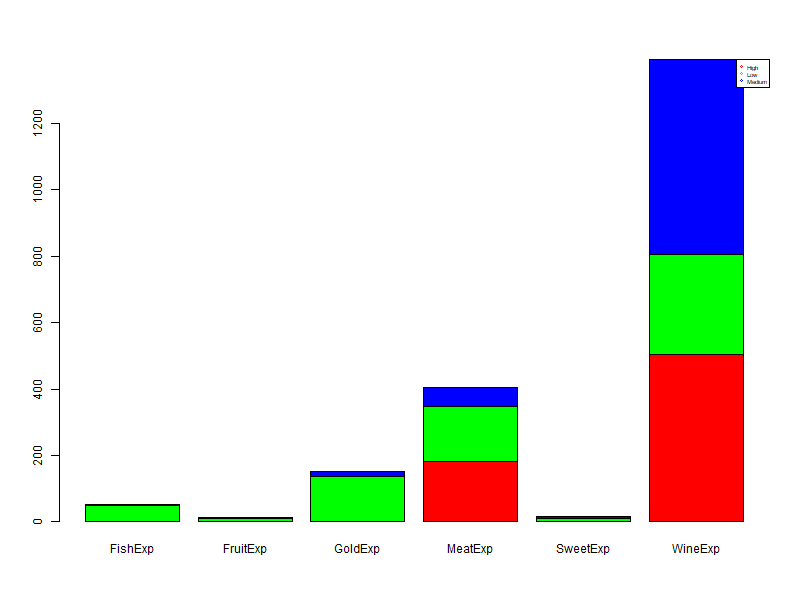
\includegraphics[width= 1\linewidth]{Imatges/stacked_barplot_counts_IncomeSegment_10_legend(category).png}
    \caption{Preferred Product Category by Income Segment}
    \label{fig:scree_plot_11} % Changed label to be unique
\end{figure}

This chart illustrates preferred product categories, broken down by income segment. 
\begin{itemize}
    \item \textbf{WineExp:} This is overwhelmingly the most preferred category across all segments, as shown by the towering bar. The largest single group of wine consumers by count is the \textbf{Low-income segment} (blue, approx. 500 counts), followed by the High-income segment (red, approx. 490 counts), and then the Medium-income segment (green, approx. 300 counts).
    \item \textbf{MeatExp:} This is the second most popular category. It is clearly dominated by the \textbf{High-income segment} (red).
    \item \textbf{Other Categories:} The remaining, less-preferred categories ('FishExp', 'FruitExp', 'GoldExp', 'SweetExp') are predominantly preferred by \textbf{Low-income} (blue) and \textbf{Medium-income} (green) consumers.
\end{itemize}

\newpage
\subsection{Conclusions}
After profiling some variables and comparing them with the clusters, we have concluded that our variables can be distributed similarly to the three main clusters.

The first cluster would represent the minority customers:
Cluster 1: Low-value customers
This group includes consumers with low or lower-middle incomes, limited education (basic or second-cycle), and children. They have more rational and restricted consumption habits, so their main purchases vary. This cluster prefers shopping through promotions or in-store.

In summary, this cluster consists of consumers with lower purchasing power, clearly oriented toward saving and seeking promotions. Their behavior reflects high price sensitivity and low brand loyalty. The most effective marketing strategies should focus on periodic promotions, engaging digital campaigns, and loyalty programs with points or discounts that encourage repeat purchases.

The second cluster represents intermediate consumers:
Cluster 2 – Mid-value customers
These consumers are characterized by having medium incomes and medium to high education levels (Graduation or Master’s). This group maintains a balance between purchase frequency and value, prefers shopping in-store or online, and their most frequently purchased products are wine and meat.

In summary, this segment shows greater stability and willingness to engage with the brand compared to Cluster 1. It represents a strategic group for loyalty and multi-channel marketing actions, as it combines digital habits with trust in the physical shopping experience. Personalized campaigns or segmented discounts can significantly increase their average value.

Finally, the third cluster concentrates the High-value customers
Cluster 3 – High-value customers
These consumers stand out for their high income levels and advanced education (Master’s or PhD). They are mostly individuals without children, which allows them to spend more on purchases. This group prefers to shop mainly in-store or through catalogs, and their most frequently purchased product is wine.

In summary, Cluster 3 represents the most profitable customers for the company. They show consistent purchasing habits, lower price sensitivity, and a preference for personalized experiences. This makes them the top priority for retention strategies and premium loyalty programs. The most effective actions are those that strengthen their connection with the brand, such as exclusive benefits, catalog offers, and direct, personalized communication.

To summarize, our database contains information on three types of customers. To maximize the potential benefit from each, we should design personalized offers with different objectives:

Cluster 1: Focus acquisition strategies on competitive pricing and digital promotions.
Cluster 2: Strengthen loyalty and multi-channel personalization.
Cluster 3: Reinforce the connection through premium experiences and exclusive services.
